In this chapter, we evaluate the \cnine and \chef symbolic execution platforms by answering the following questions: (1) What real-world software can the two platforms target? (2) Are the test cases generated effective for bug finding or achieving high coverage? (3) How efficient are the two platforms with respect to the resources used?

\section{Prototypes}

\subsection{Cloud9}

\stefan{Expand on this, after refactoring the Cloud9 chapter. Mention that the prototype is a parallel symbolic execution engine.}

We developed a \cnine prototype on top of the \klee~\cite{klee} symbolic execution engine.  The prototype has 7 \kloc.
%
The \klee modifications to support the symbolic OS abstractions amount to roughly 2 \kloc, while the rest consists of the POSIX model built on top of the abstractions.

\subsection{Chef}

\begin{figure}
  \centering
  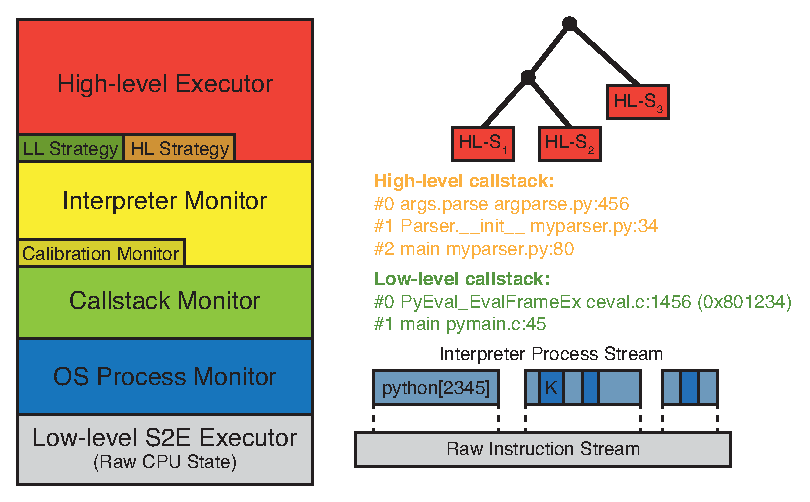
\includegraphics[width=0.7\textwidth]{figures/evaluation/chef-implem-stack}
  \caption{The implementation of \chef, as a stack of S2E analysis modules that refine the raw stream of x86 instructions into a high-level symbolic execution view.}
  \label{fig:eval:chef-implem-stack}
\end{figure}

We used \chef to generate symbolic execution engines for Python (Section~\ref{sec:python}) and Lua (Section~\ref{sec:lua}). Table~\ref{tab:pychanges} summarizes the effort to set up the two interpreters for \chef.  The necessary changes to the interpreter amount to 321 lines of code for Python and 277 for Lua.
%
The total developer time was 5 person-days for Python and 3 person-days for Lua, which is orders of magnitude smaller than the effort required for building a complete symbolic execution engine from scratch.  

\begin{table}
\centering
\small
\begin{tabular}{|@{\hspace*{4pt}}l@{\hspace*{4pt}}|@{\hspace*{4pt}}r@{\hspace*{4pt}}|@{\hspace*{4pt}}r@{\hspace*{4pt}}|}
\hline
\textbf{Component} & \textbf{Python} & \textbf{Lua}\\
\hline
Interpreter core size (C LoC) & 427,435 & 14,553 \\
\hline
\hline
HLPC instrumentation (C LoC) & 47 (0.01\%) & 44 (0.30\%) \\
Sym. optimizations (C LoC) & 274 (0.06\%) & 233 (1.58\%) \\
\hline
Native extensions (C LoC) & 1,320 (0.31\%) & 154 (1.06\%) \\
Test library (Python/Lua LoC) & 103 & 87 \\
\hline
\hline
Developer time (person-days) & 5 & 3 \\
\hline
\end{tabular}
\caption{Summary of the effort required to support Python and Lua in \chef.  The first row is the interpreter size without the standard language library. The next two rows are changes in the interpreter core, while the following two constitute the symbolic test library.  The last item indicates total developer effort.}
\label{tab:pychanges}
\end{table}

\subsubsection{Symbolic Execution Engine for Python}
\label{sec:python}

\paragraph{Interpreter Instrumentation}

We instrumented the CPython interpreter 2.7.3 for use with \chef, according to the guidelines presented in Section~\ref{sec:chef:recipe}.

Python programs are composed of modules, corresponding to Python source files.  Each source file is compiled into an interpreter-specific bytecode format, i.e., each source statement is translated into one or more lower-level primitive instructions.  The instructions are grouped into blocks, corresponding to a single loop nesting, function, method, class, or global module definition.
%
We define an \hlpc as the concatenation of the unique block address of the top frame on the stack and the current instruction offset inside the block. We instrumented the Python interpreter to pass this program location to \chef; this required adding less than 50 LoC to the main interpreter loop.

We performed several optimizations on the Python interpreter: we neutralized the hash functions of strings and integers, which are the most common objects; we concretized the memory sizes passed to the garbage-collected memory allocator; and we eliminated interning for small integers and strings.    
%
Most optimizations involved only adding preprocessor directives for conditional compilation of blocks of code.
%
We gathered the optimizations under a new \codebit{--with-symbex} flag of the interpreter's \codebit{./configure} script.

\paragraph{Symbolic Tests}

To validate the usefulness of the resulting symbolic execution engine, we use it as a test case generation tool.  To this end, we implemented a symbolic test library as a separate Python package, used both inside the guest virtual machine, and outside, during test replay.
%
Figure~\ref{fig:sample-test} is an example of a symbolic test class for the \codebit{argparse} command-line interface generator. It sets up a total of 12 symbolic characters of input: two 3-character symbolic arguments to configure the command-line parser plus another two to exercise the parsing functionality.

The test class derives from the library's \codebit{SymbolicTest} class, which provides two methods to be overridden: \codebit{setUp}, which is run once before the symbolic test starts, and \codebit{runTest}, which creates the symbolic input and can check properties.  The symbolic inputs are created by calling the \codebit{getString} and \codebit{getInt} methods in the \codebit{SymbolicTest} API.

\begin{figure}
  \centering
  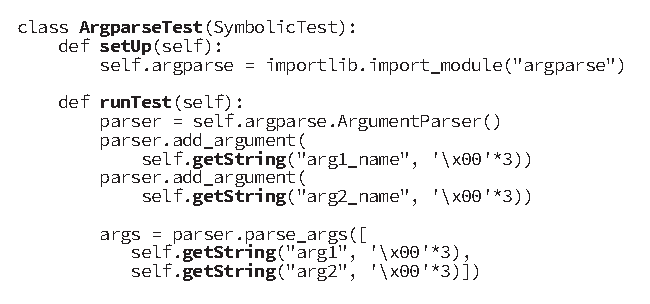
\includegraphics[width=3.2in]{figures/evaluation/symtest}
  \caption{The symbolic test used to exercise the functionality of the Python \codebit{argparse} package.}
  \label{fig:sample-test}
\end{figure}

A symbolic test is executed by a symbolic test runner, which is also part of the library.  The runner can work in either symbolic or replay mode. 
%
In \emph{symbolic mode}, the runner executes inside the guest virtual machine.  It creates a single instance of the test class, whose \codebit{getString} and \codebit{getInt} methods create corresponding Python objects and invoke the \codebit{make\_symbolic} call to mark their memory buffers as symbolic.
%
In \emph{replay mode}, the runner creates one instance of the test class for each test case created by \chef. The \codebit{getString} and \codebit{getInt} methods return the concrete input assignment of the test case.


\subsubsection{Symbolic Execution Engine for Lua}
\label{sec:lua}

Lua is a lightweight scripting language mainly used as an interpreter library to add scripting capabilities to software written in other languages. However, it also has a standalone interpreter and several Lua-only projects exist. We generated a symbolic execution engine for Lua based on version 5.2.2 of the Lua interpreter.

\paragraph{Interpreter Instrumentation}

Similar to Python, Lua programs are composed of one or more Lua source files, compiled into a bytecode format.  The code is compiled into a set of functions that operate on a global stack of values.  Each function is composed of a sequence of bytecode instructions, where each instruction is defined by an offset, opcode, and parameters.
%
We construct the \hlpc as the concatenation of the unique address of the function in the top frame and the current instruction offset being executed.  The instrumentation amounts to less than 50 LoC added to the interpreter loop.

We optimized the Lua interpreter for symbolic execution by eliminating string interning.  In addition, we configured the interpreter to use integer numbers instead of the default floating point, for which S2E does not support symbolic expressions.  This change was easy, because it was available as a macro definition in the interpreter's configuration header.

%%%%%%%%%%%%%%%%%%%%%%%%%%%%%%%%%%%%%%%%%%%%%%%%%%%%%%%%%%%%%%%%%%%%%%%%%%%%%%%%

\section{Experimental Setup and Testing Targets}

\subsection{Running Low-level Systems with Cloud9}

For all our \cnine experiments, we ran \cnine in parallel symbolic execution mode in a heterogeneous cluster environment, with worker CPU frequencies between 2.3--2.6 GHz and with 4--6 GB of RAM available per core.

On each worker, the underlying \klee engine used the best searchers from \cite{klee}, namely an interleaving of random-path and coverage-optimized strategies. At each step, the engine alternately selects one of these heuristics to pick the next state to explore. Random-path traverses the execution tree starting from the root and randomly picks the next descendant node, until a candidate state is reached. The coverage-optimized strategy weighs the states according to an estimated distance to an uncovered line of code, and then randomly selects the next state according to these weights.

To quantify coverage, we report both line coverage and path coverage numbers. Line coverage measures the fraction of program statements executed during a test run, while path coverage reports how many execution paths were explored during a test. Path coverage is the more relevant metric when comparing thoroughness of testing tools.  Nevertheless, we also evaluate properties related to line coverage, since this is still a de facto standard in software testing practice. Intuitively, and confirmed experimentally, path coverage in \cnine scales linearly with the number of workers.

Table~\ref{table:tested} shows a selection of the systems we tested with \cnine, covering several types of software.  We confirmed that each system can be tested properly under our POSIX model. In the rest of this section, we focus our in-depth evaluation on several networked servers and tools, as they are frequently used in settings where reliability matters.

\begin{table}[h!]
\addtolength{\tabcolsep}{-2pt}
\centering
\small
\begin{tabular}{| l | r@{.}p{1pt} | l |}
\hline
\textbf{~~~~~~~System} & \multicolumn{2}{|l|}{\textbf{Size (\kloc)}} & \textbf{~~~~Type of Software} \\
\hline
Apache httpd 2.2.16 & ~~~~~~~226 & 4 & \multirow{3}{*}{Web servers}\\
Lighttpd 1.4.28         &                 39 & 5 & \\
Ghttpd 1.4.4             &                   0 & 6  & \\ \hline
Memcached 1.4.5     &                   8 & 3 &  Distributed object cache \\\hline
Python 2.6.5             &               388 & 3 & Language interpreter \\ \hline
Curl 7.21.1               &                  65 & 9 & \multirow{2}{*}{Network utilities} \\ 
Rsync 3.0.7               &                  35 & 6 & \\\hline 
Pbzip 2.1.1               &                  3 & 6 & Compression utility \\ \hline
Libevent 1.4.14         &                  10 & 2 & Event notification library \\ \hline
Coreutils 6.10          &                  72 & 1 & Suite of system utilities \\ \hline
Bandicoot 1.0           &                   6 & 4 & Lightweight DBMS \\ \hline
\end{tabular}
\caption{Representative selection of testing targets that run on \cnine.  Size was measured using the \codebit{sloccount} utility.}
\label{table:tested}
\end{table}

Due to its comprehensive POSIX model, \cnine can test many kinds of servers.  One example is lighttpd, a web server used by numerous high-profile web sites, such as YouTube, Wikimedia, Meebo, and SourceForge.  For lighttpd, \cnine proved that a certain bug fix was incorrect, and the bug could still manifest even after applying the patch (Section~\ref{sec:eval:lighttpd}). \cnine also found a bug in curl, an Internet transfer application that is part of most Linux distributions and other operating systems (Section~\ref{sec:curl}).  \cnine also found a hang bug in the UDP handling code of memcached, a distributed memory object cache system used by many Internet services, such as Flickr, Craigslist, Twitter, and Livejournal (Section~\ref{sec:memcached}).

In addition to the testing targets mentioned above, we also tested a benchmark consisting of a multi-threaded and multi-process producer-consumer simulation. The benchmark exercises the entire functionality of the POSIX model: threads, synchronization, processes, and networking. 

We conclude that \cnine is practical and capable of testing a wide range of real-world software systems.


\subsection{Targeting Python and Lua Packages with Chef}

All reported \chef experiments were performed on a 48-core 2.3 GHz AMD Opteron 6176 machine with 512 GB of RAM, running Ubuntu 12.04. Each \chef invocation ran on 1 CPU core and used up to 8 GB of RAM on average.

\paragraph{Testing Targets}

\begin{table*}[!ht]
\centering
\footnotesize
\begin{tabular}{@{\hspace*{5pt}}l@{\hspace*{11pt}}r@{\hspace*{11pt}}l@{\hspace*{11pt}}l|r|c|c@{\hspace*{5pt}}}
\textbf{Package} & \textbf{LOC} & \textbf{Type} & \textbf{Description} & \textbf{Coverable LOC} & \textbf{Exceptions} & \textbf{Hangs}\\
\hline
\rule{0pt}{12pt}\textbf{Python} & & & & & \\
argparse$^{*}$ & 1,466 & System & Command-line interface & 1,174 & 4 / 0 & --- \\
ConfigParser$^{*}$ & 451 & System & Configuration file parser & 145 & 1 / 0 & --- \\
%
HTMLParser$^{*}$ & 623 & Web & HTML parser & 582 & 1 / 0 & --- \\
simplejson 3.10 & 1,087 & Web & JSON format parser & 315 & 2 / 0 & --- \\
%% webapp2 2.5.2 & 1,986 & Web & Web framework & & \\
%
unicodecsv 0.9.4 & 126 & Office & CSV file parser & 95 & 1 / 0 & --- \\
xlrd 0.9.2 & 7,241 & Office & Microsoft Excel reader & 4,914 & 5 / 4 & --- \\[2pt]
%
\hline
\rule{0pt}{12pt}\textbf{Lua} & & & & & & \\
cliargs 2.1-2 & 370 & System & Command-line interface & 273 & --- & --- \\
haml 0.2.0-1 & 984 & Web & HTML description markup & 775 & --- & --- \\
sb-JSON v2007 & 454 & Web & JSON format parser & 329 & --- & $\checkmark$ \\
markdown 0.32 & 1,057 & Web & Text-to-HTML conversion & 673 & --- & --- \\
moonscript 0.2.4-1 & 4,634 & System & Language that compiles to Lua & 3,577 & --- & --- \\[2pt]
%
\hline
\rule{0pt}{12pt}\textbf{TOTAL} & 18,493 & & & 12,852 & & \\
\end{tabular}
\caption{Summary of testing results for the Python and Lua packages
  used for evaluation. Items with (*) represent standard library
  packages.
  Exception numbers indicate total / undocumented exception types
  discovered.}
\label{tab:targets}
\end{table*}

We evaluated the symbolic execution engines for Python and Lua on 6 Python and 5 Lua packages, respectively, including system, web, and office libraries. In total, the tested code in these packages amounts to about $12.8$ KLOC.  We chose the latest versions of widely used packages from the Python standard library, the Python Package Index, and the Luarocks repository.  Whenever possible, we chose the pure interpreted implementation of the package over the native optimized one (e.g., the Python \codebit{simplejson} package). The first five columns of Table~\ref{tab:targets} summarize the package characteristics; LOC numbers were obtained with the \codebit{cloc} tool~\cite{cloc}.

The reported package sizes exclude libraries, native extension modules, and the packages' own test suites.
However, the packages ran in their unmodified form, using all the language features and libraries they were designed to use, including classes, built-in data structures (strings, lists, dictionaries), regular expressions, native extension modules, and reflection.  

All testing targets have a significant amount of their functionality written in the interpreted language itself; we avoided targets that are just simple wrappers around native extension modules (written in C or C++) in order to focus on the effectiveness of \chef at distilling high-level paths from low-level symbolic execution.  Nevertheless, we also included libraries that depend on native extension modules.  For instance, all the testing targets containing a lexing and parsing component use Python's standard regular expression library, which is implemented in C.
% The execution of parsers heavily depends on possible regular expression matches on input strings.
To thoroughly test these parsers, it is important to also symbolically execute the native regular expression library. For this, the binary symbolic execution capabilities of \chef are essential.

\paragraph{Methodology: Symbolic Tests}

For each package, we wrote a symbolic test that invokes the package's entry points with one or more symbolic strings.  
%The symbolic tests invoke the code under test in a generic manner without specific checks.  
Figure~\ref{fig:sample-test} in Section~\ref{sec:python} is an example of such a symbolic test.

Each symbolic test ran for 30 minutes within \chef, after which we replayed the collected high-level tests on the host machine, in a vanilla Python/Lua environment, to confirm test results and measure line coverage.  To compensate for the randomness in the state selection strategies, we repeated each experiment 15 times.  In each graph we present average values and error margins as +/- one standard deviation.

For our experiments, we did not use explicit specifications, but relied on generic checks for finding common programming mistakes.  For both Python and Lua, we checked for interpreter crashes and potential hangs (infinite loops). 
For Python---which, unlike Lua, has an exception mechanism---we also flagged whenever a test case led to unspecified exceptions being thrown.
%
In general, one could find application-specific types of bugs by adding specifications in the form of assertions, as in normal unit tests.

\paragraph{Methodology: Coverage Measurement}

Line or statement coverage remains widely used, even though its meaningfulness as a metric for test quality is disputed. We measure and report line coverage to give a sense of what users can expect from a test suite generated fully automatically by a symbolic execution engine based on \chef.  For Python, we rely on the popular \codebit{coverage} package, and for Lua we use the \codebit{luacov} package.

Since our prototype only supports strings and integers as symbolic program inputs, we count only the lines of code that can be reached using such inputs. We report this number as ``coverable LOC'' in the fifth column of Table~\ref{tab:targets}, and use it in our experiments as a baseline for what such a symbolic execution engine could theoretically cover directly.  For example, for the \codebit{simplejson} library, this includes only code that decodes JSON-encoded strings, not code that takes a JSON object and encodes it into a string. Note that, in principle, such code could still be tested and covered by writing a more elaborate symbolic test that sets up a JSON object based on symbolic primitives~\cite{paas-testing}.

%%%%%%%%%%%%%%%%%%%%%%%%%%%%%%%%%%%%%%%%%%%%%%%%%%%%%%%%%%%%%%%%%%%%%%%%%%%%%%%%

\section{Cloud9's Effectiveness as a Testing Platform}

In this section we present several case studies that illustrate how \cnine can explore and find new bugs, confirm/disprove that existing bugs have been correctly fixed, and regression-test a program after it has been modified.  In the common case, \cnine users start with a concrete test case (e.g., from an existing test suite) and generalize it by making data symbolic and by controlling the environment.

%--------------------------------------------------
\subsection{Case Study \#1: Curl}
\label{sec:curl}

Curl is a popular data transfer tool for multiple network protocols, including HTTP and FTP.  When testing it, \cnine\ found a new bug which causes Curl to crash when given a URL regular expression of the form ``\codebit{http://site.\{one,\linebreak two,three\}.com\{}''. \cnine exposed a general problem in Curl's handling of the case when braces used for regular expression globbing are not matched properly.  The bug was confirmed and fixed within 24 hours by the developers. 

This problem had not been noticed before because the globbing functionality in Curl was shadowed by the same functionality in command-line interpreters (e.g., Bash).  This case study illustrates a situation that occurs often in practice: when a piece of software is used in a way that has not been tried before, it is likely to fail due to latent bugs.

\subsection{Case Study \#2: Memcached}
\label{sec:memcached}

Memcached is a distributed memory object cache system, mainly used to speed up web application access to persistent
data, typically residing in a database. % Memcached is deployed at many large sites like Facebook, Twitter, and YouTube. 

Memcached comes with an extensive test suite comprised of C and Perl code. Running it completely takes about 1 minute; it runs 6,472 different test cases  and explores $83.66\%$ of the code. While this is considered thorough by today's standards, two easy \cnine\ test cases further increased code coverage. Table~\ref{table:memcached} contains a summary of our results, presented in more details in the following paragraphs.


\paragraph{Symbolic Packets}

The memcached server accepts commands over the network. Based on memcached's C test suite, we wrote a test case that sends memcached a generic, symbolic binary command (i.e., command content is fully symbolic), followed by a second symbolic command. This test captures all operations that entail a pair of commands.

A 24-worker \cnine\ explored in less than 1 hour all 74,503 paths associated with this sequence of two symbolic packets, covering an additional 1.13\% of the  code relative to the original test suite.  What we found most encouraging in this result is that such exhaustive tests constitute first steps toward using symbolic tests to \emph{prove} properties of real-world programs, not just to look for bugs.  Symbolic tests may provide an alternative to complex proof mechanisms that is more intuitive for developers and thus more practical.

\paragraph{Symbolic Fault Injection}

We also tested memcached with fault injection enabled, whereby we injected all feasible failures in memcached's calls to the C Standard Library.  After 10 minutes of testing, a 24-worker \cnine\ explored 312,465 paths, adding $1.28\%$ over the base test suite.  The fact that {\em line} coverage increased by so little, despite having covered almost $50\times$ more paths, illustrates the weakness of line coverage as a metric for test quality---high line coverage should offer no high confidence in the tested code's quality.

For the fault injection experiment, we used a special strategy that sorts the execution states according to the number of faults recorded along their paths, and favors the states with fewer fault injection points. This led to a uniform injection of faults: we first injected one fault in every possible fault injection point along the original C test suite path, then injected pairs of faults, and so on.  We believe this is a practical approach to using fault injection as part of regular testing.

\begin{table}
\small
\centering
\addtolength{\tabcolsep}{-1.3pt}
\begin{tabular}{| p{2.3cm} | r | c | c | }
\hline
{\bf Testing Method}   & {\bf Paths}~~       & {\bf Isolated}             & {\bf Cumulated}          \\ 
                                & {\bf  Covered}  & {\bf Coverage$^{*}$} & {\bf Coverage$^{**}$}      \\
\hline
Entire test suite               & 6,472         & $83.67\%$        &---                   \\
\hline
\raggedright Binary protocol test suite      & 27            & $46.79\%$        & $84.33\%$ ($+0.67\%$) \\
\hline
Symbolic packets                & 74,503        & $35.99\%$        & $84.79\%$ ($+1.13\%$) \\
\hline
\raggedright Test suite + fault~injection    & 312,465       & $47.82\%$        & $84.94\%$ ($+1.28\%$) \\
\hline
\end{tabular}
\caption{Path and code coverage increase obtained by each symbolic testing technique on memcached. We show total coverage obtained with each testing method (*), as well as total coverage obtained by augmenting the original test suite with the indicated method  (**); in parentheses, we show the increase over the entire test suite's coverage.}
\label{table:memcached}
% \vspace{-0.3cm}
\end{table}

\paragraph{Hang Detection}

We tested memcached with symbolic UDP packets, and \cnine discovered a hang condition in the packet parsing code: 
when a sequence of packet fragments of a certain size arrive at the server, memcached enters an infinite loop, which prevents it from serving any further UDP connections. This bug can seriously hurt the availability of infrastructures using memcached.

We discovered the bug by limiting the maximum number of instructions executed per path to $5 \times 10^6$.  The paths without the bug terminated after executing $\approximately 3\times 10^5$ instructions; the other paths that hit the maximum pointed us to the bug.

%--------------------------------------------------
\subsection{Case Study \#3: Lighttpd}
\label{sec:eval:lighttpd}


The lighttpd web server is specifically engineered for high request throughput, and it is quite sensitive to the rate at which new data is read from a socket.  Alas, the POSIX specification offers no guarantee on the number of bytes that can be read from a file descriptor at a time.  lighttpd 1.4.12 has a bug in the command-processing code that causes the server to crash (and connected clients to hang indefinitely) depending on how the incoming stream of requests is fragmented. 

We wrote a symbolic test case to exercise different \emph{stream fragmentation} patterns and see how different lighttpd versions behave. We constructed a simple HTTP request, which was then sent over the network to lighttpd. We activated network packet fragmentation via the symbolic \codebit{ioctl()}  API explained in Section~\ref{sec:cloud9:platform}. We confirmed that certain fragmentation patterns cause lighttpd to crash (prior to the bug fix). However, we also tested the server right after the fix and discovered that the bug fix was incomplete, as some fragmentation patterns still cause a crash and hang the client (Table~\ref{table:lighttpd}).

This case study shows that \cnine can find bugs caused by specific interactions with the environment which are hard to test with a concrete test suite. It also shows how \cnine can be used to write effective regression test suites---had a stream-fragmentation symbolic test been run after the fix, the lighttpd developers would have promptly discovered the incompleteness of their fix.

\begin{table}
\small
\centering
\begin{tabular}{| p{3.8cm} | p{1.65cm} | p{1.65cm} |}
\hline
\bf Fragmentation pattern & \bf ver. 1.4.12 & \bf ver. 1.4.13 \\
\bf (data sizes in bytes) & \bf (pre-patch)     & \bf (post-patch)\\
\hline
$1 \times 28$ 			& 		OK		& OK \\
\hline
$1 \times 26 + 1 \times 2$  & crash + hang 	& OK \\
\hline
$2+5+1+5+2 \times 1 + 3 \times 2 + 5 + 2 \times 1 $	& crash + hang 	& crash + hang \\
\hline
\end{tabular}
\caption{The behavior of different versions of lighttpd to three ways of fragmenting the HTTP request "GET /index.html HTTP/1.0\textsc{Cr}\textsc{Lf}\textsc{Cr}\textsc{Lf}" (string length 28).}
\label{table:lighttpd}
\end{table}

\subsection{Case Study \#4: Bandicoot DBMS}
\label{sec:bandicoot}

Bandicoot is a lightweight DBMS that can be accessed over an HTTP interface.  We exhaustively explored all paths handling the GET commands and found a bug in which Bandicoot reads from outside its allocated memory.  The particular test we ran fortuitously did not result in a crash, as Bandicoot ended up reading from the libc memory allocator's metadata preceding the allocated block of memory. However, besides the read data being wrong, this bug could cause a crash depending on where the memory block was allocated.

To discover and diagnose this bug without \cnine is difficult. First, a concrete test case has little chance of triggering the bug.  Second, searching for the bug with a sequential symbolic execution tool seems impractical: the exhaustive exploration took 9 hours with a 4-worker \cnine (and less than 1 hour with a 24-worker cluster). 

\subsection{Discussion}

\cnine inherits \klee's capabilities, being able to recognize memory errors and failed assertions. We did not add much in terms of bug detection, only two mechanisms for detecting hangs: check if all symbolic threads are sleeping (deadlock) and set a threshold for the maximum number of instructions executed per path (infinite loop or livelock).  Even so, \cnine can find bugs beyond \klee's abilities because the POSIX model allows \cnine to reach more paths and explore deeper portions of the tested program's code---this exposes additional potentially buggy situations. \cnine also has more total memory and CPU available, due to its distributed nature, so it can afford to explore more paths than \klee.  As we have shown above, it is feasible to offer proofs for certain program properties: despite the exponential nature of exhaustively exploring paths, one can build small but useful symbolic test cases that can be exhaustively executed.

\section{Chef's Effectiveness for Automated Testing}
\label{sec:eval:chef-atcg}

We evaluate the effectiveness of the generated symbolic execution engines for bug detection and exception exploration.

\paragraph{Bug Detection}

The specifications we used for our experiments are application-agnostic and only check for per-path termination within a given time bound and for the absence of unrecoverable crashes.  The first specification checks whether a call into the runtime returns within 60 seconds.  In this way, we discovered a bug in the Lua JSON package that causes the parser to hang in an infinite loop: if the JSON string contains the \codebit{/*} or \codebit{//} strings marking the start of a comment but no matching \codebit{*/} or line terminator, the parser reaches the end of the string and continues spinning waiting for another token.
%
This bug is interesting for two reasons: First, comments are not part of the JSON standard, and the parser accepts them only for convenience, so this is a clear case of an interpreter-specific bug.  Second, JSON encodings are normally automatically generated and transmitted over the network, so they are unlikely to contain comments; traditional testing is thus likely to miss this problem. However, an attacker could launch a denial of service attack by sending a JSON object with a malformed comment.

The second implicit specification checks that a program never terminates non-gracefully, i.e., the interpreter implementation or a native extension crashes without giving the program a chance to recover through the language exception mechanisms.  In our experiments, our test cases did not expose any such behavior.

\paragraph{Exception Exploration}

This scenario focuses on finding undocumented exceptions in Python code.
%
Being memory-safe languages, crashes in Python and Lua code tend to be due to \emph{unhandled exceptions} rather than bad explicit pointers.  When such exceptions are not caught by the program, they propagate to the top of the stack and cause the program to be terminated prematurely. 
%
In dynamic languages, it is difficult to determine all the possible exceptions that a function can throw to the callee, because there is no language-enforced type-based API contract.  Users of an API can only rely on the documentation or an inspection of the implementation.  Therefore, undocumented exceptions are unlikely to be checked for in \codebit{try}-\codebit{except} constructs and can erroneously propagate further.
%
They can then hurt productivity (e.g., a script that crashes just as it was about to complete a multi-TB backup job) or disrupt service (e.g., result in an HTTP 500 Internal Server Error).

We looked at all the Python exceptions triggered by the test cases generated using \chef and classified them into \emph{documented} and \emph{undocumented}.  The documented exceptions are either exceptions explicitly mentioned in the package documentation or common Python exceptions that are part of the standard library (e.g., \codebit{KeyError}, \codebit{ValueError}, \codebit{TypeError}).  Undocumented exceptions are all the rest.

The sixth column in Table~\ref{tab:targets} summarizes our findings.  We found four undocumented exceptions in \codebit{xlrd}, the largest package.  These exceptions occur when parsing a Microsoft Excel file, and they are \codebit{BadZipfile}, \codebit{IndexError}, \codebit{error}, and \codebit{AssertionError}.  These errors occur inside the inner components of the Excel parser, and should have either been documented or, preferably, been caught by the parser and re-raised as the user-facing \codebit{XLRDError}.

\section{Impact of \cupa Heuristics and Interpreter Optimizations}
\label{sec:sub:perf-cupa}

We now analyze the impact of the \cupa heuristics (described in Section~\ref{sec:chef:cupa}) and the interpreter optimizations (described in Section~\ref{sec:chef:optimzeforsymbex}) on test generation effectiveness.  Specifically, we measure the number of paths (respectively source code lines) covered by the test suite generated in 30 minutes for the packages in Table~\ref{tab:targets}.

We compare the results obtained in 4 different configurations: (1) the baseline, consisting of performing random state selection while executing the unmodified interpreter, and then either use (2) the path- or coverage-optimized CUPA only, (3) the optimized interpreter only, or (4) both CUPA and the optimized interpreter.  This way we measure the individual contribution of each technique, as well as their aggregate behavior.

\paragraph{Test Case Generation}

Figure~\ref{fig:tc-improv} compares the number of test cases generated with each of the 4 \chef configurations, using the path-optimized CUPA~(Section~\ref{sec:chef:cupa-paths}).  We only count the \textit{relevant} high-level test cases, that is, each test case exercises a unique high-level path in the target Python program.

\begin{figure}[t]
  \centering
  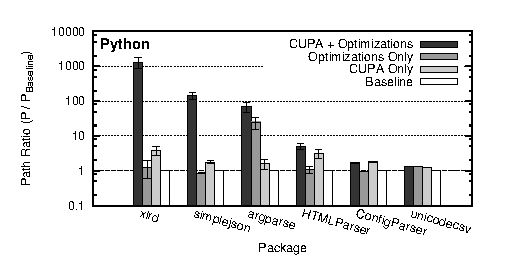
\includegraphics[width=3.27in]{figures/evaluation/bkdown-path-python} \\
  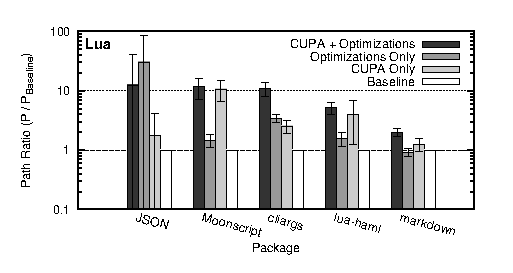
\includegraphics[width=3.27in]{figures/evaluation/bkdown-path-lua}
  \caption{The number of Python and Lua test cases generated by
    coverage- and path-optimized \cupa relative to random state
    selection (logarithmic scale).}
  \label{fig:tc-improv}
\end{figure}

For all but one of the 11 packages (6 Python plus 5 Lua), the aggregate CUPA + interpreter optimizations performs the best, often by a significant margin over the baseline.  This validates the design premises behind our techniques.

The CUPA strategy and the interpreter optimizations may interact non-linearly.  In two cases (Python's \codebit{xlrd} and \codebit{simplejson}), the aggregate significantly outperforms either individual technique. These are cases where the result is better than the sum of its parts.  In the other cases, the result is roughly the sum of each part, although the contribution of each part differs among targets.  This is visually depicted on the log-scale graph: for each cluster, the heights of the middle bars measured from level $1 \times$ roughly add up to the height of the aggregate (left) bar.

In one case (Lua's \codebit{JSON}), the aggregate performs worse on average than using the interpreter optimizations alone.  Moreover, the performance of each configuration is less predictable, as shown by the large error bars.  This behavior is due to the generated tests that cause the interpreter to hang, as explained in Section~\ref{sec:eval:chef-atcg}.  To detect hangs, the test runs for 60 seconds before switching to another test case.  This acts as a ``penalty'' for the configurations that find more paths leading to the hang and also skews the distribution of path execution times, since the hanging paths take significantly longer than the normal (terminating) paths.

\paragraph{Line Coverage}

Figure~\ref{fig:coverage-improv} shows the line coverage achieved by each configuration, using CUPA optimized for line coverage (Section~\ref{sec:chef:cupa-coverage}).  In 6 out of 11 packages, the coverage improvement is noticeable, and for Python's \codebit{simplejson} and \codebit{xlrd}, the improvements are significant ($80\%$ and $40\%$).

Note that these coverage improvements are obtained using basic symbolic tests that do not make assumptions about the input format.  We believe that tailoring the symbolic tests to the specifics of each package could improve these results significantly.

\begin{figure}[t]
  \centering
  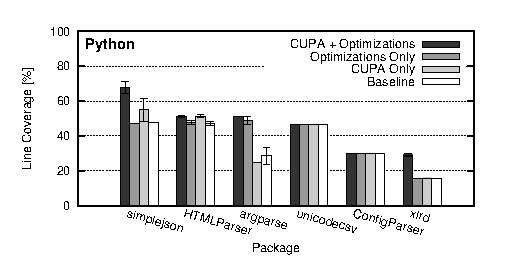
\includegraphics[width=3.2in]{figures/evaluation/bkdown-stmtcov-python} \\
  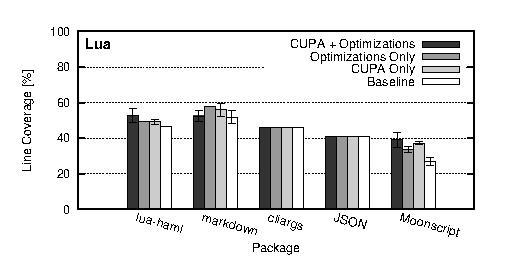
\includegraphics[width=3.2in]{figures/evaluation/bkdown-stmtcov-lua}
  \caption{Line coverage for the experiments of Figure~\ref{fig:tc-improv}.}
  \label{fig:coverage-improv}
\end{figure}

\section{Breaking Down Chef's Interpreter Optimizations}
\label{sec:sub:optimizations}

We now analyze in more depth the impact of the interpreter optimizations by breaking them down into the three types mentioned in Section~\ref{sec:chef:optimzeforsymbex}: avoiding symbolic pointers, hash neutralization, and fast-path elimination.  We run again the symbolic tests for 30 minutes, using the path-optimized CUPA and four different interpreter builds, starting from the vanilla interpreter and adding the optimization types one by one.  For each build and package, we count the number of high-level paths discovered by \chef.

Figure~\ref{fig:optimizations} shows the results for Python.  The data is normalized such that the number of high-level paths for each target reaches $100\%$.  For 3 out of 6 packages (\codebit{simplejson}, \codebit{argparse}, and \codebit{HTMLParser}), \chef's performance monotonically increases as more optimizations are introduced.  For \codebit{unicodecsv} and \codebit{ConfigParser}, the optimizations do not bring any benefits or even hurt slightly.  

However, in the case of \codebit{xlrd}, hash neutralization and fast path elimination seem to actually \emph{hurt} symbolic execution, since the best performance is attained when only symbolic pointer avoidance is in effect.  We explain this behavior by the fact that the different optimization levels cause the search strategy to explore different behaviors of the target package.  \codebit{xlrd} is by far the largest Python package in our evaluation (7.2KLOC vs. the second largest of 1.4KLOC) and includes a diverse set of behaviors, each with its own performance properties.

This result suggests that, for large packages, a \emph{portfolio} of interpreter builds with different optimizations enabled would help further increase the path coverage.

\begin{figure}
  \centering
  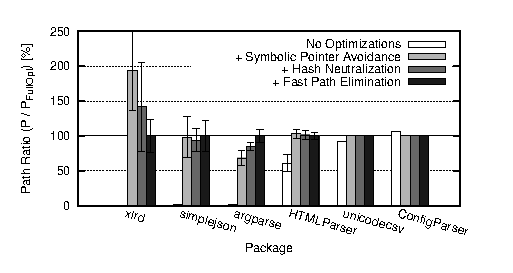
\includegraphics[width=3.2in]{figures/evaluation/optimizations-bars-python}
  \caption{The contribution of interpreter optimizations for Python as number of high-level paths explored.  Number of paths is relative to full optimizations ($100\%$) for each package.}
  \label{fig:optimizations}
\end{figure}


\section{Comparing Chef Against Hand-Made Engines}
\label{sec:sub:comparison}

We now evaluate the trade-offs in using a symbolic execution engine generated with \chef over building one ``by hand''.

\paragraph{Hand-Made Engines}

To our knowledge, no symbolic execution engine for Lua exists.  For Python, we found three research tools, which we compare \chef to.  (1) \cutiepy~\cite{cutie-py} is a concolic engine based on a formal model of the Python language.  It uses a custom CPython interpreter to drive a concrete execution, along with updating the symbolic state according to model semantics. (2) NICE-PySE~\cite{nice} is part of the NICE framework for testing OpenFlow applications.  We will refer to it as \nicese, for brevity. It wraps supported data types into symbolic counterparts that carry the symbolic store, and uses Python's tracing mechanisms to implement the interpretation loop fully in Python.  (3) The symbolic execution engine of the scalability testing tool Commuter~\cite{commuter} is also entirely built in Python.  Its primary purpose is the construction of models that explicitly use an API of symbolic data types.

We perform our comparison along three aspects: language features supported, implementation faithfulness, and performance.  The last two aspects are evaluated only against \nicese, which, besides being open source, is most compatible with our symbolic data representation (based on STP~\cite{stp}).

\paragraph{Language Feature Support}

Table~\ref{tab:langfeats} summarizes the language feature support for \chef, \nicese, \cutiepy, and \commuterse, as implemented at the moment of writing.  We relied on information from the respective papers in all cases and additionally on the implementation in the cases of \nicese and \commuterse, which are available as open source.

We distinguish engines designed to support arbitrary Python code (the ``Vanilla'' label) and those where the symbolic data types are an API used by model code (the ``Model'' label).  Engines in the ``Model'' category essentially offer a ``symbolic domain-specific language'' on top of the interpreted language.  \chef, \cutiepy, and \nicese are ``vanilla'' engines, since their testing targets do not have to be aware that they are being symbolically executed.  \commuterse is a model-based engine, since its testing targets are bound to the symbolic API offered by the engine.

We grouped the supported language features into program state representation (the language data model and types) and manipulation (the operations on data).  We divide data types into values (integers, strings and floating-point), collections (lists and dictionaries), and user-defined classes.  The operations consist of data manipulation, basic control flow (e.g., branches, method calls), advanced control flow (e.g., exception handling, generators), and native method invocations (they are atomic operations at the high level).  We also include in the comparison the ability to execute unsupported operations in concrete-only mode.


% Some names unlikely to clash with other definitions...
\newcommand{\compsupp}{\ensuremath{\CIRCLE}}
\newcommand{\partsupp}{\ensuremath{\LEFTcircle}}
\newcommand{\unsupp}{\ensuremath{\Circle}}

\begin{table}[tb]
\centering
\small
\begin{tabular}{@{\hspace*{2pt}}l@{\hspace*{2pt}} | @{\hspace*{2pt}}c@{\hspace*{2pt}} | @{\hspace*{2pt}}c@{\hspace*{2pt}} | @{\hspace*{2pt}}c@{\hspace*{2pt}} | @{\hspace*{2pt}}c@{\hspace*{2pt}}}
                    & \textbf{\chef}            & \textbf{\cutiepy} & \textbf{\nicese} & \textbf{\commuterse} \\
\hline
\rule{0pt}{12pt}\textbf{Engine type}& Vanilla   & Vanilla    & Vanilla   & Model       \\
\rule{0pt}{12pt}\textbf{Data types} &           &            &           &             \\
Integers            & $\compsupp^{\hphantom{*}}$  & \compsupp  & \compsupp  & \compsupp  \\
Strings             & $\compsupp^{\hphantom{*}}$  & \unsupp    & \unsupp    & \partsupp  \\
Floating point      & $\unsupp^{\hphantom{*}}$    & \unsupp    & \unsupp    & \unsupp    \\
Lists and maps      & $\compsupp^{*}$           & \partsupp   & \unsupp    & \compsupp  \\
User-defined classes& $\compsupp^{*}$           & \unsupp     & \partsupp   & \partsupp \\
\rule{0pt}{12pt}\textbf{Operations}   &                          &            &            &             \\
Data manipulation     & $\compsupp^{\hphantom{*}}$ & \partsupp  &  \partsupp & \partsupp   \\
Basic control flow    & $\compsupp^{\hphantom{*}}$ & \compsupp  &  \partsupp & \compsupp   \\
Advanced control flow & $\compsupp^{\hphantom{*}}$ & \compsupp  &  \unsupp   & \compsupp   \\
Native methods        & $\compsupp^{\hphantom{*}}$ & \partsupp  &  \unsupp   & \unsupp     \\
\end{tabular}
\rule{0pt}{12pt}\compsupp Complete \hspace{12pt} \partsupp Partial \hspace{12pt} \unsupp Not supported
\caption{Language feature support comparison for \chef and dedicated Python symbolic execution engines.  %% A full bullet means complete concrete and symbolic support for the feature available in the implementation.  A half-full bullet means a partial implementation, while an empty bullet means no support for the feature.
  Complete support with (*) refers to the internal program data flow and not to the initial symbolic variables.}
\label{tab:langfeats}
\end{table}

In a nutshell, \cutiepy is able to complete correctly any execution in concrete mode by using the interpreter implementation directly.   However, the symbolic semantics for each data type and native function must be explicitly provided by the developer, which makes \cutiepy impractical to use with rich Python applications.  \nicese suffers from the additional limitation that it has to support each bytecode instruction explicitly, which makes the tool impossible to use beyond its target applications.  Finally, \commuterse provides a rich set of symbolic data types, including lists and maps, by taking advantage of Z3's extended support for arrays~\cite{general-arrays}.  However, it supports only Python programs explicitly written against its API and does not handle native functions.

%% \cutiepy supports the semantics of integers, maps, and lists.  Other data types are supported as uninterpreted types, whose objects are opaque except for their identity.  Other data structures may be added to the model, expressed as uninterpreted functions and arrays.  By using the interpreter implementation to drive the concrete execution, \cutiepy is able to complete correctly any execution in concrete mode, while the symbolic evaluation and branching is limited to what the model offers.

%% \nicese supports only integers and Ethernet frame headers (encapsulated in a class) as symbolic data types, since they are required by the targeted OpenFlow switch applications.  Similarly, the supported operations include those encountered in the target applications.  This leaves out the support for advanced control flow and native methods (other than the built-in calls required by the supported data types).  By using its own (incomplete) interpretation loop, \nicese is not able to fall back on concretizing unsupported operations and so terminates the execution with an error in such cases.

%% \commuterse takes advantage of Z3's extended support for arrays~\cite{general-arrays} to efficiently model lists and maps, in addition to integers.  The support for strings is partially provided by uninterpreted types, which can only reason about object equality.  Moreover, the uninterpreted types can be used as keys in symbolic maps, which allows data structures such as file directories used in the POSIX model.

The engine generated by \chef offers complete symbolic support for almost all language features.  Floating point operations are supported only concretely, due to lack of support in STP, the constraint solver used by S2E.  For the same reasons, the symbolic program inputs can only be integers and strings.  However, all data structures are supported during the execution.

Each half or empty bullet in Table~\ref{tab:langfeats} implies that significant engineering effort would be required to complete a feature.  While useful for their evaluation targets, \nicese and \cutiepy are unable to handle a complex software package that makes use of Python's many language features.


\paragraph{Use as Reference Implementation}

When the need for performance justifies investing in a dedicated engine implementation, an engine created from \chef can serve as a reference implementation during development.  One can find bugs in a symbolic execution engine by comparing its test cases with those generated by \chef.  The process can be automated by tracking the test cases generated by the target engine along the high level paths generated by \chef to determine duplicates and missed feasible paths.

%% To automate the engine comparison, we augmented \chef with test case ``seeding''. The tests generated with the target engine (\nicese) are fed to \chef as ``seeds'',  which are tracked along the high-level paths generated by \chef.  A seed test follows a high-level path if the test input matches the path constraint.  If the target engine is correct, each \chef high-level path should track exactly one seed.  More seeds per path indicate test case duplication, while zero seeds flags a missed path.

In this mode, we found a bug in the \nicese implementation, which was causing it to generate redundant test cases and miss feasible paths.  The bug was in the way \nicese handled \codebit{if not <expr>} statements in Python, causing the engine to select for exploration the wrong branch alternate and end up along an old path.  We are assisting the \nicese developers in identifying and fixing any other such bugs.

In conclusion, the experiment provides evidence that a system combining an established low-level symbolic execution engine (e.g., S2E) with a reference interpreter implementation is more robust than a symbolic execution engine built from scratch.


%% \johannes{This entire section is strange, because we evaluate this only for NICE, whereas we claimed initially that we would evaluate correctness against all engines}


\paragraph{Performance}

The downside of \chef is that the symbolic execution engines produced are slower than their hand-written equivalents.  We quantify this drawback by applying \chef to the experimental setup of \nicese, consisting of an OpenFlow switch controller program that implements a MAC learning algorithm.  The controller receives as input a sequence of Ethernet frames and, in response, updates its forwarding table (stored as a Python dictionary).  We use symbolic tests that supply sequences of between 1 and 10 Ethernet frames, each having the MAC address and frame types marked as symbolic.

\begin{figure}
  \centering
  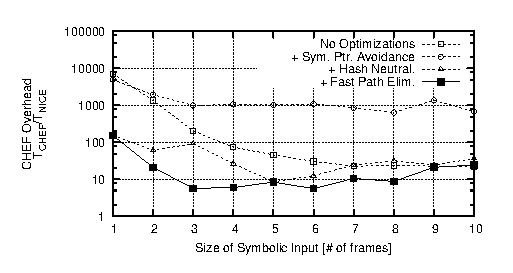
\includegraphics[width=3.2in]{figures/evaluation/nice-optimizations}
  \caption{Average overhead of \chef compared to \nicese, computed as ratio of average per-path execution times.  The average divides total tool execution time by number of high-level paths generated.}
  \label{fig:nice-overhead}
\end{figure}

Given the small size of the controller (less than 100~LOC), the number of execution paths is relatively small, and choosing low-level paths at random quickly discovers new high-level paths.  Therefore, the search strategy has no impact (in the experiments we used path-optimized CUPA).  However, the interpreter optimizations are crucial, since the controller code relies heavily on the dictionary.  As in Section~\ref{sec:sub:optimizations}, we use several interpreter builds with optimizations introduced one-by-one.

Figure~\ref{fig:nice-overhead} illustrates the overhead for each optimization configuration, as a function of number of Ethernet frames supplied.  The overhead is computed as the ratio between the average execution times per high-level path of \nicese and \chef.  In turn, the execution time per high-level path is computed by dividing the entire execution time of each tool by the number of paths it produced.

%% Basically the same reasons we already gave earlier in the paper

The performance of each optimization configuration illustrates the sources of path explosion and slowdown in the vanilla interpreter.  With no optimizations, symbolic keys in the MAC dictionary cause massive path explosion due to symbolic pointers.  When avoiding symbolic pointers, performance drops even more due to symbolic hash computations.  This penalty is reduced up to two orders of magnitude with hash neutralization.  Finally, fast path elimination reduces the forking inside string key comparisons in the dictionary.

The shape of the final performance curve (the solid line) is convex.  For 1 and 2 symbolic frames, the search space is quickly exhausted and the execution time is dominated by \chef's initialization costs, i.e., setting up the symbolic VM and executing the interpreter initialization inside the guest.  This results in an execution overhead as high as $120 \times$.  For more symbolic frames, the initialization cost is amortized, and the overhead goes below $5 \times$.  However, as the number of frames increases, so does the length of the execution paths and the size of the path constraints, which deepens the gap between \chef's low-level reasoning and \nicese's higher level abstractions.  For 10 symbolic frames, the overhead is around $40 \times$.

Despite \chef's performance penalty, the alternative of writing an engine by hand is daunting. It involves developing explicit models that, for a language like Python, are expensive, error-prone, and require continuous adjustments as the language evolves.
%
Where performance is crucial, a hand-written engine is superior; however, we believe that \chef is a good match in many cases.


%% \section{Scalability Analysis}

%% Discuss scalability of the Cloud9 parallelization algorithm.

%% Discuss overhead of Chef compared to hand-written engines.

%%% Local Variables: 
%%% mode: latex
%%% eval: (visual-line-mode)
%%% fill-column: 1000000
%%% TeX-master: "main"
%%% End:
